%%%%%%%%%%%%
%
% $Autor: Wings $
% $Datum: 2019-03-05 08:03:15Z $
% $Pfad: MainFunction.tex $
% $Version: 4250 $
% !TeX spellcheck = en_GB/de_DE
% !TeX encoding = utf8
% !TeX root = manual 
% !TeX TXS-program:bibliography = txs:///biber
%
%%%%%%%%%%%%

\chapter{Hauptfunktion}
\begin{figure}[ht]
	\centering
	% Erstes Bild
	\begin{minipage}[b]{0.48\textwidth}
		\centering
		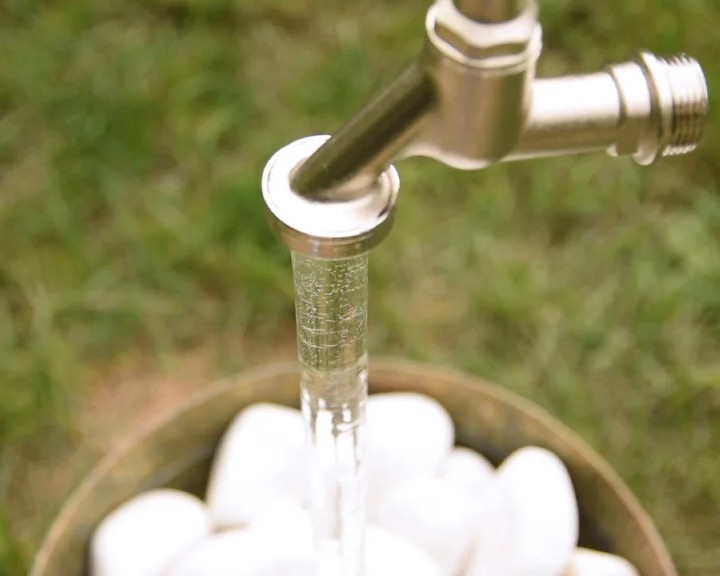
\includegraphics[width=6.5cm]{General/wasserhahn1.jpg}
		\caption{Schwebender Effekt}
		\label{fig:wasserhahn1}
	\end{minipage}
	%\hspace{0.04\textwidth} % Kleiner Abstand zwischen den Bildern
	% Zweites Bild
	\begin{minipage}[b]{0.48\textwidth}
		\centering
		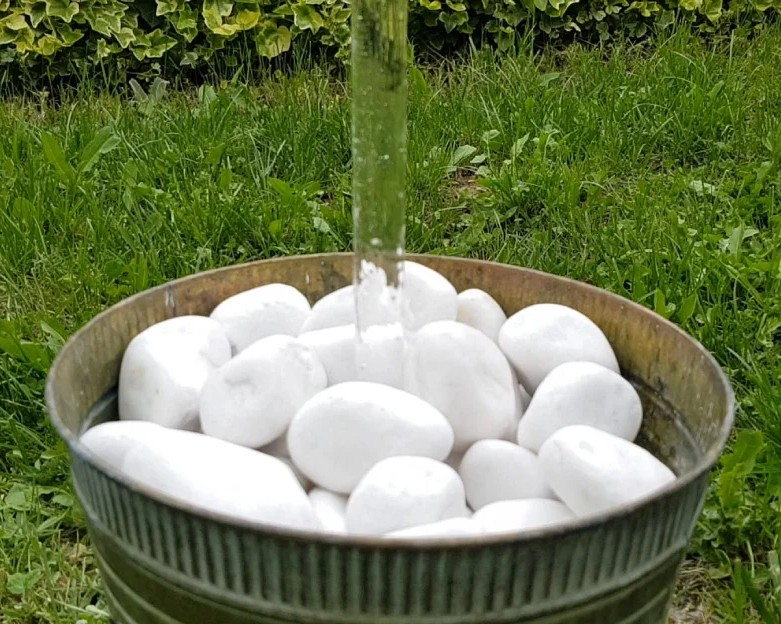
\includegraphics[width=6.5cm]{General/wasserhahn2.jpg}
		\caption{Dekorative Steine}
		\label{fig:wasserhahn2}
	\end{minipage}
\end{figure}
Der Magic Faucet Fountain erzeugt die Illusion, wie in \ref{fig:wasserhahn1} zu sehen, in der ein Wasserhahn durch eine Wassersäule in der Luft gehalten wird. Der Wasserhahn \glqq schwebt\grqq  auf dem Wasser mithilfe eines Acryl-Rohres und begießt die dekorativen Steine, wie in \ref{fig:wasserhahn2} zu sehen ist.